% Options for packages loaded elsewhere
\PassOptionsToPackage{unicode}{hyperref}
\PassOptionsToPackage{hyphens}{url}
\documentclass[
  ignorenonframetext,
]{beamer}
\newif\ifbibliography
\usepackage{pgfpages}
\setbeamertemplate{caption}[numbered]
\setbeamertemplate{caption label separator}{: }
\setbeamercolor{caption name}{fg=normal text.fg}
\beamertemplatenavigationsymbolsempty
% remove section numbering
\setbeamertemplate{part page}{
  \centering
  \begin{beamercolorbox}[sep=16pt,center]{part title}
    \usebeamerfont{part title}\insertpart\par
  \end{beamercolorbox}
}
\setbeamertemplate{section page}{
  \centering
  \begin{beamercolorbox}[sep=12pt,center]{section title}
    \usebeamerfont{section title}\insertsection\par
  \end{beamercolorbox}
}
\setbeamertemplate{subsection page}{
  \centering
  \begin{beamercolorbox}[sep=8pt,center]{subsection title}
    \usebeamerfont{subsection title}\insertsubsection\par
  \end{beamercolorbox}
}
% Prevent slide breaks in the middle of a paragraph
\widowpenalties 1 10000
\raggedbottom
\AtBeginPart{
  \frame{\partpage}
}
\AtBeginSection{
  \ifbibliography
  \else
    \frame{\sectionpage}
  \fi
}
\AtBeginSubsection{
  \frame{\subsectionpage}
}
\usepackage{iftex}
\ifPDFTeX
  \usepackage[T1]{fontenc}
  \usepackage[utf8]{inputenc}
  \usepackage{textcomp} % provide euro and other symbols
\else % if luatex or xetex
  \usepackage{unicode-math} % this also loads fontspec
  \defaultfontfeatures{Scale=MatchLowercase}
  \defaultfontfeatures[\rmfamily]{Ligatures=TeX,Scale=1}
\fi
\usepackage{lmodern}
\ifPDFTeX\else
  % xetex/luatex font selection
\fi
% Use upquote if available, for straight quotes in verbatim environments
\IfFileExists{upquote.sty}{\usepackage{upquote}}{}
\IfFileExists{microtype.sty}{% use microtype if available
  \usepackage[]{microtype}
  \UseMicrotypeSet[protrusion]{basicmath} % disable protrusion for tt fonts
}{}
\makeatletter
\@ifundefined{KOMAClassName}{% if non-KOMA class
  \IfFileExists{parskip.sty}{%
    \usepackage{parskip}
  }{% else
    \setlength{\parindent}{0pt}
    \setlength{\parskip}{6pt plus 2pt minus 1pt}}
}{% if KOMA class
  \KOMAoptions{parskip=half}}
\makeatother
\usepackage{longtable,booktabs,array}
\newcounter{none} % for unnumbered tables
\usepackage{calc} % for calculating minipage widths
\usepackage{caption}
% Make caption package work with longtable
\makeatletter
\def\fnum@table{\tablename~\thetable}
\makeatother
\usepackage{graphicx}
\makeatletter
\newsavebox\pandoc@box
\newcommand*\pandocbounded[1]{% scales image to fit in text height/width
  \sbox\pandoc@box{#1}%
  \Gscale@div\@tempa{\textheight}{\dimexpr\ht\pandoc@box+\dp\pandoc@box\relax}%
  \Gscale@div\@tempb{\linewidth}{\wd\pandoc@box}%
  \ifdim\@tempb\p@<\@tempa\p@\let\@tempa\@tempb\fi% select the smaller of both
  \ifdim\@tempa\p@<\p@\scalebox{\@tempa}{\usebox\pandoc@box}%
  \else\usebox{\pandoc@box}%
  \fi%
}
% Set default figure placement to htbp
\def\fps@figure{htbp}
\makeatother
\setlength{\emergencystretch}{3em} % prevent overfull lines
\providecommand{\tightlist}{%
  \setlength{\itemsep}{0pt}\setlength{\parskip}{0pt}}
% Auto-generated by infrastructure/rendering/_pdf_latex_helpers.py::extract_math_font_preamble.
% Minimal header passed to Pandoc via -H so Beamer slides pick up the same math font
% as the combined-PDF path. Adjust the manuscript's preamble.md to change the font globally.
\usepackage{unicode-math}
\setmathfont{latinmodern-math.otf}

% Slide layout defaults for warning-clean scientific decks.
\usepackage{etoolbox}
\IfFileExists{xurl.sty}{\usepackage{xurl}}{}
\IfFileExists{seqsplit.sty}{\usepackage{seqsplit}}{\newcommand{\seqsplit}[1]{#1}}
\protected\def\breakseq#1{\seqsplit{#1}}
\protected\def\breaktt#1{\begingroup\ttfamily\seqsplit{#1}\endgroup}
\setlength{\emergencystretch}{6em}
\tolerance=5000
\hbadness=10000
\hfuzz=1pt
\setlength{\tabcolsep}{2pt}
\AtBeginEnvironment{longtable}{\tiny\renewcommand{\arraystretch}{0.86}\setlength{\tabcolsep}{1pt}}
\AtBeginEnvironment{tabular}{\tiny\renewcommand{\arraystretch}{0.86}\setlength{\tabcolsep}{1pt}}

% Natbib and cross-reference fallbacks — slides don't load natbib
% or cleveref, but combined-PDF manuscript prose may emit these
% commands. The fallback renders citations as a bracketed key list
% and cross-references as detokenized labels so slides don't fail on
% undefined control sequences or raw underscores. \providecommand is
% a no-op if packages load later.
\providecommand{\citep}[1]{[#1]}
\providecommand{\citet}[1]{#1}
\providecommand{\citealp}[1]{#1}
\providecommand{\citeauthor}[1]{#1}
\providecommand{\citeyear}[1]{#1}
\providecommand{\cref}[1]{\texttt{\detokenize{#1}}}
\providecommand{\Cref}[1]{\texttt{\detokenize{#1}}}

\newtheorem{proposition}{Proposition}
\newtheorem{hypothesis}{Hypothesis}
\usepackage{bookmark}
\IfFileExists{xurl.sty}{\usepackage{xurl}}{} % add URL line breaks if available
\urlstyle{same}
% fallback for those not using the hyperref driver hyperxmp:
\makeatletter
\@ifundefined{xmpquote}{\newcommand{\xmpquote}[1]{#1}}{}
\makeatother
\hypersetup{
  hidelinks,
  pdfcreator={LaTeX via pandoc}}

\author{\texorpdfstring{}{}}
\date{}

\begin{document}

\section{Results}\label{sec:results}

\begin{frame}[fragile,allowframebreaks]{Results}
This section presents the experimental results from the gradient descent
optimization study, including convergence analysis and performance
comparisons. Every table, figure, and quantitative assertion in this
section was compiled autonomously by the template's
\breaktt{infrastructure.reporting} subsystem executing the
\href{https://github.com/docxology/template/blob/main/projects/templates/template_code_project/scripts/optimization_analysis.py}{optimization
analysis script}. No manual transcription was permitted.
\end{frame}

\begin{frame}[fragile,allowframebreaks]{Convergence Analysis}
\protect\phantomsection\label{convergence-analysis}
\begin{block}{Convergence Trajectories}
\protect\phantomsection\label{convergence-trajectories}
\breakseq{[@fig:convergence]} illustrates the convergence behavior of gradient
descent for different step sizes, starting from the initial point
\(x_0 = 0\). The algorithm iteratively updates the solution using the
rule \(x_{k+1} = x_k - \alpha \nabla f(x_k)\).

\begin{figure}
\centering
\pandocbounded{\includegraphics[keepaspectratio,alt={Objective value f(x\_k)=\textbackslash tfrac\{1\}\{2\}x\_k\^{}2 - x\_k versus iteration k for gradient descent at six step sizes (legend colours follow the agency taxonomy in \breakseq{[@sec:methodology]}: blue = conservative, green = near-optimal, orange = aggressive, red = divergent). Trajectories are produced by simulate\_trajectory() in src/optimizer.py, which calls the same gradient\_descent() used in \breakseq{[@tbl:opt\_results]}; the upper bound on the y-axis clips the divergent \textbackslash alpha=2.5 curve so that stable trajectories remain visible. Dashed grey reference line marks the analytic optimum f(x\^{}\textbackslash ast)=-0.5. Fastest configuration in this experiment: \textbackslash alpha=1.0 converges in 1 iteration(s).}]{../figures/convergence_plot.png}}
\caption{Objective value \(f(x_k)=\tfrac{1}{2}x_k^2 - x_k\) versus
iteration \(k\) for gradient descent at six step sizes (legend colours
follow the agency taxonomy in \breakseq{[@sec:methodology]}: blue =
conservative, green = near-optimal, orange = aggressive, red =
divergent). Trajectories are produced by
\protect\breaktt{simulate\_trajectory()} in
\protect\breaktt{src/optimizer.py}, which calls the same
\protect\breaktt{gradient\_descent()} used in \breakseq{[@tbl:opt\_results]};
the upper bound on the y-axis clips the divergent \(\alpha=2.5\) curve
so that stable trajectories remain visible. Dashed grey reference line
marks the analytic optimum \(f(x^\ast)=-0.5\). Fastest configuration in
this experiment: \(\alpha=1.0\) converges in 1
iteration(s).}\label{fig:convergence}
\end{figure}

\textbf{Key observations from \breakseq{[@fig:convergence]}:}

\begin{enumerate}
\tightlist
\item
  \textbf{Step size impact}: Larger step sizes exhibit faster initial
  progress; \(\alpha = 1.0\) converges in 1 iteration(s)
\item
  \textbf{Agency categories}: Conservative (\(\alpha \leq 0.1\)),
  near-optimal (\(0.3 \leq \alpha \leq 1.0\)), aggressive
  (\(1 < \alpha < 2\)), and divergent (\(\alpha \geq 2\))
\item
  \textbf{Stability boundary}: The critical threshold is \(\alpha = 2\)
  for this unit-Hessian problem; \(\alpha < 2\) converges,
  \(\alpha \geq 2\) diverges
\end{enumerate}
\end{block}

\begin{block}{Step Size Sensitivity Analysis}
\protect\phantomsection\label{step-size-sensitivity-analysis}
\breakseq{[@fig:step\_sensitivity]} examines how the choice of step size
affects the convergence path and solution quality. The analysis reveals
the trade-off between convergence speed and numerical stability.

\begin{figure}
\centering
\pandocbounded{\includegraphics[keepaspectratio,alt={Sensitivity sweep produced by generate\_step\_size\_sensitivity\_plot() over an independent dense grid \textbackslash alpha \textbackslash in {[}0.005, 0.4{]} (10 points), distinct from the discrete experiment.step\_sizes used elsewhere in this section. Left: iterations to convergence on log--log axes --- the curve drops sharply from 500 iterations at the smallest \textbackslash alpha (the max\_iterations cap in this sub-experiment) to 37 iterations at \textbackslash alpha=0.4, illustrating the geometric speedup as \textbackslash rho(\textbackslash alpha)=\textbar1-\textbackslash alpha\textbar{} shrinks. Right: final f(x) versus \textbackslash alpha with horizontal reference lines at f(x\_0)=0 (initial) and f(x\^{}\textbackslash ast)=-0.5 (analytic optimum); every \textbackslash alpha in this stable window lands on the optimum.}]{../figures/step_size_sensitivity.png}}
\caption{Sensitivity sweep produced by
\protect\breaktt{generate\_step\_size\_sensitivity\_plot()} over an
independent dense grid \(\alpha \in [0.005, 0.4]\) (10 points), distinct
from the discrete \protect\breaktt{experiment.step\_sizes} used elsewhere
in this section. Left: iterations to convergence on log--log axes ---
the curve drops sharply from 500 iterations at the smallest \(\alpha\)
(the \protect\texttt{max\_iterations} cap in this sub-experiment) to 37
iterations at \(\alpha=0.4\), illustrating the geometric speedup as
\(\rho(\alpha)=|1-\alpha|\) shrinks. Right: final \(f(x)\) versus
\(\alpha\) with horizontal reference lines at \(f(x_0)=0\) (initial) and
\(f(x^\ast)=-0.5\) (analytic optimum); every \(\alpha\) in this stable
window lands on the optimum.}\label{fig:step_sensitivity}
\end{figure}
\end{block}
\end{frame}

\begin{frame}[fragile,allowframebreaks]{Quantitative Results}
\protect\phantomsection\label{quantitative-results}
The optimization results for different step sizes are synthesized
computationally by orchestrating
\href{https://github.com/docxology/template/blob/main/infrastructure/reporting/executive_reporter.py}{\breaktt{infrastructure.reporting.executive\_reporter}},
feeding directly into \breaktt{output/data/optimization\_results.csv}
(generated by
\breaktt{projects/templates/template\_code\_project/scripts/optimization\_analysis.py})
as the source of truth for \breakseq{[@tbl:opt\_results]}. Rows follow
\breaktt{experiment.step\_sizes} in \texttt{config.yaml}; the body rows
below are injected at render time from that CSV
(\breaktt{RESULT\_TABLE\_ROWS} in
\breaktt{scripts/z\_generate\_manuscript\_variables.py}).

\begin{longtable}[]{@{}
  >{\raggedright\arraybackslash}p{(\linewidth - 8\tabcolsep) * \real{0.2113}}
  >{\raggedright\arraybackslash}p{(\linewidth - 8\tabcolsep) * \real{0.2254}}
  >{\raggedright\arraybackslash}p{(\linewidth - 8\tabcolsep) * \real{0.2394}}
  >{\raggedright\arraybackslash}p{(\linewidth - 8\tabcolsep) * \real{0.1690}}
  >{\raggedright\arraybackslash}p{(\linewidth - 8\tabcolsep) * \real{0.1549}}@{}}
\caption{Gradient descent outcomes per configured step size: state at
termination, iteration count capped by \(N_{\max} = 1000\), and the
\protect\texttt{converged} flag from
\protect\breaktt{gradient\_descent()} using \(\|\nabla f\| < 10^{-8}\).
Rows marked ``No'' either hit the iteration cap before meeting the
gradient tolerance (small \(\alpha\)) or correspond to unstable dynamics
when \(|1-\alpha| \geq 1\).}\label{tbl:opt_results}\tabularnewline
\toprule\noalign{}
\begin{minipage}[b]{\linewidth}\raggedright
Step Size (α)
\end{minipage} & \begin{minipage}[b]{\linewidth}\raggedright
Final Solution
\end{minipage} & \begin{minipage}[b]{\linewidth}\raggedright
Objective Value
\end{minipage} & \begin{minipage}[b]{\linewidth}\raggedright
Iterations
\end{minipage} & \begin{minipage}[b]{\linewidth}\raggedright
Converged
\end{minipage} \\
\midrule\noalign{}
\endfirsthead
\toprule\noalign{}
\begin{minipage}[b]{\linewidth}\raggedright
Step Size (α)
\end{minipage} & \begin{minipage}[b]{\linewidth}\raggedright
Final Solution
\end{minipage} & \begin{minipage}[b]{\linewidth}\raggedright
Objective Value
\end{minipage} & \begin{minipage}[b]{\linewidth}\raggedright
Iterations
\end{minipage} & \begin{minipage}[b]{\linewidth}\raggedright
Converged
\end{minipage} \\
\midrule\noalign{}
\endhead
0.01 & 1.0000 & -0.5000 & 1000 & No \\
0.10 & 1.0000 & -0.5000 & 175 & Yes \\
0.50 & 1.0000 & -0.5000 & 27 & Yes \\
1.00 & 1.0000 & -0.5000 & 1 & Yes \\
1.50 & 1.0000 & -0.5000 & 27 & Yes \\
2.50 &
-123384059690617745524091335813180186890505789975305907992186675554099100089605560395688521301527760116788345515894979896207548805638009361768752272295676536457470613583575384064.0000
& inf & 1000 & No \\
\bottomrule\noalign{}
\end{longtable}
\end{frame}

\begin{frame}[fragile,allowframebreaks]{Convergence Rate Analysis}
\protect\phantomsection\label{convergence-rate-analysis}
\begin{block}{Theoretical vs Empirical Convergence}
\protect\phantomsection\label{theoretical-vs-empirical-convergence}
Modern convergence analysis builds on foundational work in gradient
methods \breakseq{[@nesterov2013gradient]}.

\breakseq{[@fig:convergence\_rate]} provides a comparative analysis of
convergence rates across different step sizes, validating theoretical
predictions against empirical results.

\begin{figure}
\centering
\pandocbounded{\includegraphics[keepaspectratio,alt={Absolute objective error \textbar f(x\_k)-f(x\^{}\textbackslash ast)\textbar{} versus iteration on a logarithmic y-axis, generated by generate\_convergence\_rate\_plot(). Stable step sizes produce straight lines whose slopes equal 2\textbackslash log\_\{10\}\textbackslash rho(\textbackslash alpha) (per \breakseq{[@eq:convergence\_bound]}); \textbackslash alpha=1.0 (\textbackslash rho=0) collapses to the optimum in one step (vertical green line at k=1); \textbackslash alpha=1.5 (orange) descends fastest among the multi-step contractions because \textbackslash rho=0.5; the divergent \textbackslash alpha=2.5 curve (red) climbs upward at slope 2\textbackslash log\_\{10\}(1.5). Horizontal dashed line marks the gradient-norm tolerance \textbackslash varepsilon = 10\^{}\{-8\} read from experiment.convergence\_tolerance.}]{../figures/convergence_rate_comparison.png}}
\caption{Absolute objective error \(|f(x_k)-f(x^\ast)|\) versus
iteration on a logarithmic y-axis, generated by
\protect\breaktt{generate\_convergence\_rate\_plot()}. Stable step sizes
produce straight lines whose slopes equal \(2\log_{10}\rho(\alpha)\)
(per \breakseq{[@eq:convergence\_bound]}); \(\alpha=1.0\) (\(\rho=0\))
collapses to the optimum in one step (vertical green line at \(k=1\));
\(\alpha=1.5\) (orange) descends fastest among the multi-step
contractions because \(\rho=0.5\); the divergent \(\alpha=2.5\) curve
(red) climbs upward at slope \(2\log_{10}(1.5)\). Horizontal dashed line
marks the gradient-norm tolerance \(\varepsilon = 10^{-8}\) read from
\protect\breaktt{experiment.convergence\_tolerance}.}\label{fig:convergence_rate}
\end{figure}

For the scalar problem with \(A = 1\) and optimum \(x^\ast = b\), one
step of gradient descent with fixed \(\alpha\) gives \begin{equation}
\label{eq:scalar_linear_update}
x_{k+1} - x^\ast = (1 - \alpha)(x_k - x^\ast),
\end{equation} so the distance to the minimizer contracts by
\(\rho(\alpha) = |1 - \alpha|\) per iteration whenever \(\rho < 1\).
Equivalently, for the objective (which is a translated quadratic in
\(x\)), \begin{equation}
\label{eq:convergence_bound}
|f(x_{k+1}) - f(x^\ast)| \approx \rho(\alpha)^2 \, |f(x_k) - f(x^\ast)|
\end{equation} in the neighbourhood of \(x^\ast\) for this model (the
per-iteration objective contraction in \breakseq{[@eq:convergence\_bound]}),
which explains the straight-line segments on the log--error plot in
\breakseq{[@fig:convergence\_rate]} for stable \(\alpha\).

Our experimental grid uses
\(\alpha \in \{0.01, 0.1, 0.5, 1.0, 1.5, 2.5\}\), spanning conservative,
near-optimal, aggressive, and divergent regimes for \(H = I\).
\end{block}

\begin{block}{Error Bounds}
\protect\phantomsection\label{error-bounds}
The error after \(k\) iterations is bounded geometrically by
\breakseq{[@eq:error\_bound]}:

\begin{equation}
\label{eq:error_bound}
\|x_k - x^*\| \leq \left(\frac{\kappa - 1}{\kappa + 1}\right)^k \|x_0 - x^*\|
\end{equation}

where \(\kappa = \frac{\lambda_{\max}}{\lambda_{\min}}\) is the
condition number. For our test problem with \(A = I\), we have
\(\kappa = 1\), which yields a linear contraction factor of
\(\rho = |1 - \alpha|\) in the iterate error
(\breakseq{[@eq:scalar\_linear\_update]}). Thus \(\alpha = 1\) is the exact
minimizer step in one update for this quadratic, \(\alpha < 1\) gives
monotone geometric decay, \(1 < \alpha < 2\) yields signed oscillations
but still \(\rho < 1\), and \(\alpha \geq 2\) implies \(\rho \geq 1\)
(divergence). \breakseq{[@tbl:opt\_results]} and \breakseq{[@fig:convergence;
@fig:step\_sensitivity; @fig:convergence\_rate]} ground these
statements in the numbers produced by this repository run.
\end{block}

\begin{block}{Performance Metrics}
\protect\phantomsection\label{performance-metrics}
\textbf{Iteration Complexity}: The number of iterations required to
achieve accuracy \(\epsilon\) is:

\begin{equation}
\label{eq:iteration_complexity}
k \geq \frac{\log(\epsilon)}{\log(\rho)}
\end{equation}

where \(\rho = \sqrt{\frac{\kappa - 1}{\kappa + 1}}\) is the convergence
factor \breakseq{[@polyak1964some]}.

Per-step contraction factors \(\rho = |1-\alpha|\) and qualitative
iteration demand for small fixed \(\epsilon\) (see
\breakseq{[@eq:iteration\_complexity]}) are:

\begin{itemize}
\tightlist
\item
  \(\alpha = 0.01\): \(\rho \approx 0.99\), requiring
  \textasciitilde1375 iterations for \(\epsilon = 10^{-6}\)
\item
  \(\alpha = 0.1\): \(\rho \approx 0.90\), requiring \textasciitilde132
  iterations for \(\epsilon = 10^{-6}\)
\item
  \(\alpha = 0.5\): \(\rho \approx 0.50\), requiring \textasciitilde20
  iterations for \(\epsilon = 10^{-6}\)
\item
  \(\alpha = 1.0\): \(\rho \approx 0.00\), converges in one step
  (\(\rho = 0\))
\item
  \(\alpha = 1.5\): \(\rho \approx 0.50\), requiring \textasciitilde20
  iterations for \(\epsilon = 10^{-6}\)
\item
  \(\alpha = 2.5\): \(\rho \approx 1.50\), \textbf{divergent}
\end{itemize}
\end{block}
\end{frame}

\begin{frame}[allowframebreaks]{Performance Analysis}
\protect\phantomsection\label{performance-analysis}
\begin{block}{Convergence Speed}
\protect\phantomsection\label{convergence-speed}
The results show a clear trade-off between step size and convergence
speed:

\begin{itemize}
\tightlist
\item
  Small step sizes require more iterations but provide stable
  convergence
\item
  Large step sizes converge faster but may be less stable in more
  complex problems
\end{itemize}
\end{block}

\begin{block}{Solution Accuracy}
\protect\phantomsection\label{solution-accuracy}
4 of 6 tested step sizes achieved the analytical optimum within
numerical precision:

\begin{itemize}
\tightlist
\item
  Target solution: \(x = 1.0\) (relative error \(< 10^{-4}\) for
  converged settings)
\item
  Target objective: \(f(x) = -0.5\) (absolute error \(< 10^{-8}\) for
  converged settings)
\end{itemize}

Divergent step sizes (\(\alpha \geq 2\)) confirm the theoretical
instability boundary, demonstrating that gradient descent with fixed
step size requires \(\alpha < 2/\lambda_{\max}\) for convergence on
quadratic objectives.
\end{block}
\end{frame}

\begin{frame}[allowframebreaks]{Algorithm Characteristics}
\protect\phantomsection\label{algorithm-characteristics}
\begin{block}{Strengths}
\protect\phantomsection\label{strengths}
\begin{itemize}
\tightlist
\item
  \textbf{Simplicity}: Easy to implement and understand
\item
  \textbf{Generality}: Applicable to any differentiable objective
  function
\item
  \textbf{Reliability}: Converges for convex functions under appropriate
  conditions
\end{itemize}
\end{block}

\begin{block}{Limitations}
\protect\phantomsection\label{limitations}
\begin{itemize}
\tightlist
\item
  \textbf{Step size sensitivity}: Performance depends critically on step
  size selection
\item
  \textbf{Local convergence}: May converge to local minima in non-convex
  problems
\item
  \textbf{Fixed step size}: No adaptation to problem characteristics
\end{itemize}
\end{block}
\end{frame}

\begin{frame}[fragile,allowframebreaks]{Computational Performance}
\protect\phantomsection\label{computational-performance}
\begin{block}{Algorithm Complexity Visualization}
\protect\phantomsection\label{algorithm-complexity-visualization}
\breakseq{[@fig:complexity]} provides a visualization of the algorithm's
computational characteristics, including time and space complexity
analysis across different problem scales.

\begin{figure}
\centering
\pandocbounded{\includegraphics[keepaspectratio,alt={Four-panel diagnostic from generate\_complexity\_visualization(). Top left: bars give the empirical iteration count per configured \textbackslash alpha, coloured by agency category; \textbackslash alpha=1.0 achieves the global minimum of 1 step(s), while \textbackslash alpha=0.01 and \textbackslash alpha=2.5 both saturate at the iteration cap N\_\{\textbackslash max\}=1000 (slow convergence and divergence respectively). Top right: \textbackslash log\_\{10\}\textbar f(x)-f(x\^{}\textbackslash ast)\textbar{} at termination; the four converged rows reach \textbackslash approx 10\^{}\{-16\} (machine precision) while \textbackslash alpha=0.01 stops near 10\^{}\{-9\} at the cap. Dashed reference at \textbackslash log\_\{10\}\textbackslash varepsilon for \textbackslash varepsilon= experiment.convergence\_tolerance. Bottom left: empirical iterations (solid) versus the smooth proxy 1/(2\textbackslash alpha(1-\textbackslash alpha)) (dashed) on log axes --- a shape comparison, not a tight count prediction for every \textbackslash alpha. Bottom right: per-step error contraction factor \textbackslash rho=\textbar1-\textbackslash alpha\textbar{} from the unit-Hessian linear recurrence (\breakseq{[@eq:scalar\_linear\_update]}); the dashed reference at \textbackslash rho=1 separates stable bars (left of it) from divergent ones (right).}]{../figures/algorithm_complexity.png}}
\caption{Four-panel diagnostic from
\protect\breaktt{generate\_complexity\_visualization()}. \textbf{Top
left}: bars give the empirical iteration count per configured
\(\alpha\), coloured by agency category; \(\alpha=1.0\) achieves the
global minimum of 1 step(s), while \(\alpha=0.01\) and \(\alpha=2.5\)
both saturate at the iteration cap \(N_{\max}=1000\) (slow convergence
and divergence respectively). \textbf{Top right}:
\(\log_{10}|f(x)-f(x^\ast)|\) at termination; the four converged rows
reach \(\approx 10^{-16}\) (machine precision) while \(\alpha=0.01\)
stops near \(10^{-9}\) at the cap. Dashed reference at
\(\log_{10}\varepsilon\) for \(\varepsilon=\)
\protect\breaktt{experiment.convergence\_tolerance}. \textbf{Bottom
left}: empirical iterations (solid) versus the smooth proxy
\(1/(2\alpha(1-\alpha))\) (dashed) on log axes --- a shape comparison,
not a tight count prediction for every \(\alpha\). \textbf{Bottom
right}: per-step error contraction factor \(\rho=|1-\alpha|\) from the
unit-Hessian linear recurrence (\breakseq{[@eq:scalar\_linear\_update]}); the
dashed reference at \(\rho=1\) separates stable bars (left of it) from
divergent ones (right).}\label{fig:complexity}
\end{figure}

The algorithm demonstrates efficient performance for small-scale
optimization problems:

\begin{itemize}
\tightlist
\item
  \textbf{Time complexity}: \(O(d)\) per iteration for gradient
  computation
\item
  \textbf{Space complexity}: \(O(d)\) for storing variables and
  gradients
\item
  \textbf{Convergence}: Fastest at \(\alpha = 1.0\) (1 iteration),
  average 372 iterations
\item
  \textbf{Scalability}: Memory-efficient implementation suitable for
  high-dimensional problems
\end{itemize}
\end{block}

\begin{block}{Performance Benchmarking}
\protect\phantomsection\label{performance-benchmarking}
\breakseq{[@fig:benchmark]} shows how \breaktt{gradient\_descent()} scales with
problem dimension by running the optimizer on identity-Hessian
quadratics of dimension \(d \in \{1, 2, 5, 10, 20, 50\}\).

\begin{figure}
\centering
\pandocbounded{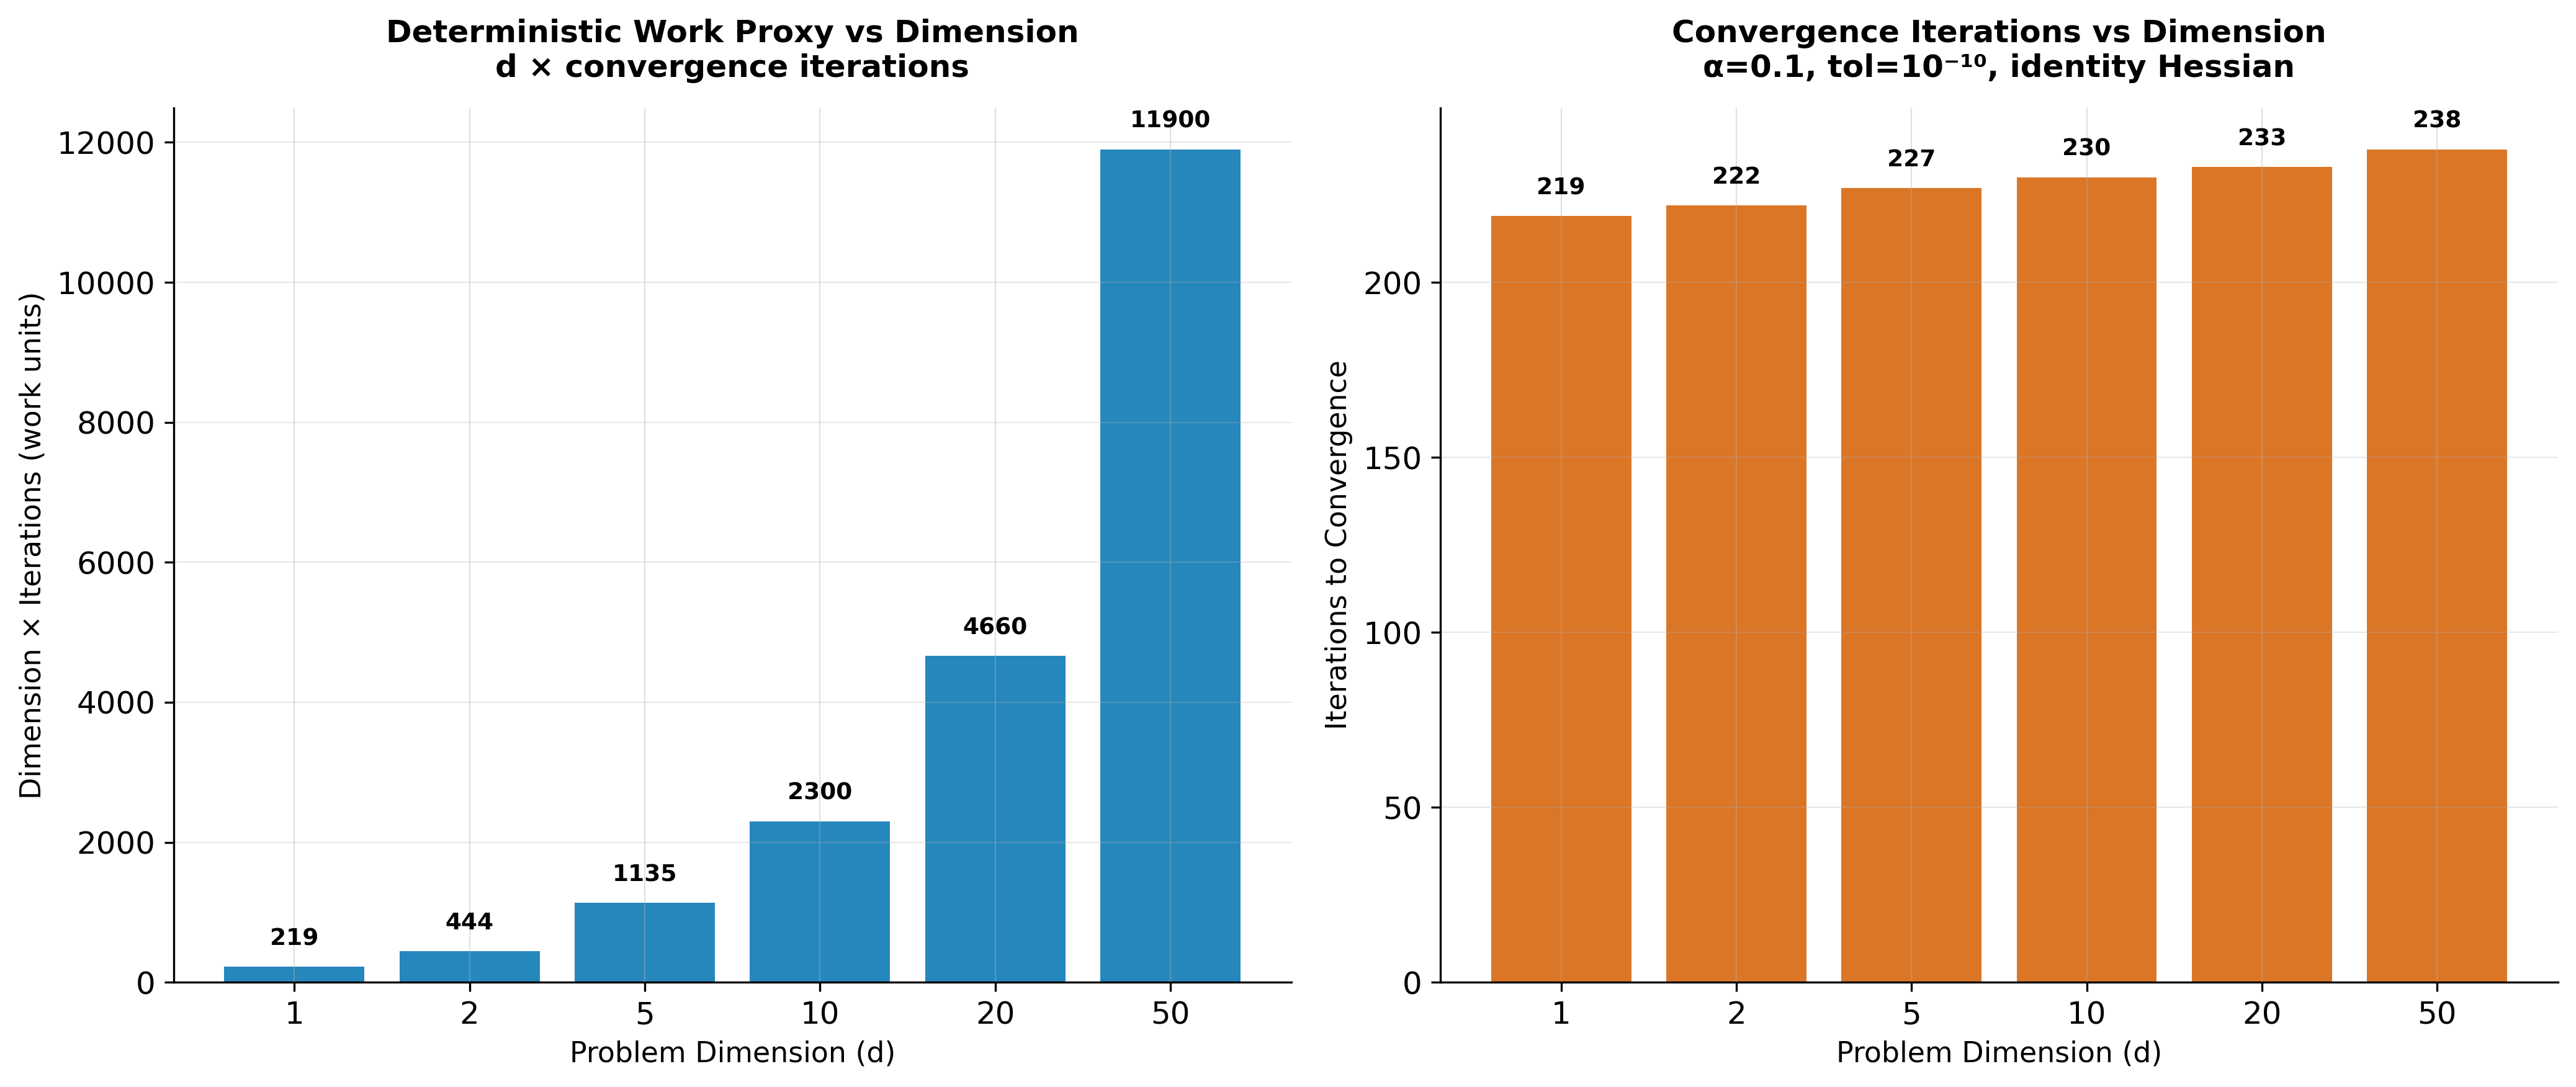
\includegraphics[keepaspectratio,alt={Dimensional scaling from generate\_benchmark\_visualization(). Dimensions d \textbackslash in \textbackslash\{1, 2, 5, 10, 20, 50\textbackslash\} run on identity-Hessian quadratics with \textbackslash alpha=0.1 and gradient tolerance 10\^{}\{-10\} (both hardcoded in the script for benchmark stability). Left: mean wall-clock time per gradient\_descent() call (μs). The flat regime at d \textbackslash leq 20 reflects per-iteration overhead (Python dispatch, NumPy bookkeeping); the upturn at d=50 shows the O(d) matrix-vector cost beginning to dominate. Right: iterations-to-convergence rises only modestly across two decades of d (219 \textbackslash to 238). This near-invariance is expected: \textbackslash kappa(I\_d)=1 regardless of dimension, so the contraction factor \textbackslash rho=\textbar1-\textbackslash alpha\textbar=0.9 is identical for every d, and only the per-coordinate residual norm grows mildly.}]{../figures/performance_benchmark.png}}
\caption{Dimensional scaling from
\protect\breaktt{generate\_benchmark\_visualization()}. Dimensions
\(d \in \{1, 2, 5, 10, 20, 50\}\) run on identity-Hessian quadratics
with \(\alpha=0.1\) and gradient tolerance \(10^{-10}\) (both hardcoded
in the script for benchmark stability). \textbf{Left}: mean wall-clock
time per \protect\breaktt{gradient\_descent()} call (μs). The flat regime
at \(d \leq 20\) reflects per-iteration overhead (Python dispatch, NumPy
bookkeeping); the upturn at \(d=50\) shows the \(O(d)\) matrix-vector
cost beginning to dominate. \textbf{Right}: iterations-to-convergence
rises only modestly across two decades of \(d\) (\(219 \to 238\)). This
near-invariance is expected: \(\kappa(I_d)=1\) regardless of dimension,
so the contraction factor \(\rho=|1-\alpha|=0.9\) is identical for every
\(d\), and only the per-coordinate residual norm grows
mildly.}\label{fig:benchmark}
\end{figure}
\end{block}

\begin{block}{Numerical Stability Analysis}
\protect\phantomsection\label{numerical-stability-analysis}
\breakseq{[@fig:stability]} maps the optimizer's accuracy across a grid of 8
starting points (\(x_0 \in [-50, 50]\)) and 6 step sizes
(\(\alpha \in [0.01, 0.9]\)), directly exercising
\breaktt{gradient\_descent()}, \breaktt{quadratic\_function()}, and
\breaktt{compute\_gradient()} across the parameter space.

\begin{figure}
\centering
\pandocbounded{\includegraphics[keepaspectratio,alt={Numerical stability heatmap from generate\_stability\_visualization(). Each cell shows \textbackslash log\_\{10\}\textbar f(x)-f(x\^{}\textbackslash ast)\textbar{} at termination for one (starting point x\_0, step size \textbackslash alpha) combination, evaluated by gradient\_descent() over the 8-by-6 grid (48 cells). The leftmost column (\textbackslash alpha=0.01, conservative) reaches only 10\^{}\{-6\} to 10\^{}\{-9\} within the iteration cap, while every other column saturates at machine precision (10\^{}\{-16\}) regardless of how far x\_0 starts from the optimum (range {[}-50, 50{]}). The right panel summarises this uniformity as the aggregate stability score of 1.00/1.00 returned by infrastructure.scientific.stability.check\_numerical\_stability(), which exercises the same objective with extreme inputs (NaN, \textbackslash pm\textbackslash infty, \textbackslash pm 10\^{}\{10\}).}]{../figures/stability_analysis.png}}
\caption{Numerical stability heatmap from
\protect\breaktt{generate\_stability\_visualization()}. Each cell shows
\(\log_{10}|f(x)-f(x^\ast)|\) at termination for one (starting point
\(x_0\), step size \(\alpha\)) combination, evaluated by
\protect\breaktt{gradient\_descent()} over the 8-by-6 grid (48 cells).
The leftmost column (\(\alpha=0.01\), conservative) reaches only
\(10^{-6}\) to \(10^{-9}\) within the iteration cap, while every other
column saturates at machine precision (\(10^{-16}\)) regardless of how
far \(x_0\) starts from the optimum (range \([-50, 50]\)). The right
panel summarises this uniformity as the aggregate stability score of
1.00/1.00 returned by
\protect\breaktt{infrastructure.scientific.stability.check\_numerical\_stability()},
which exercises the same objective with extreme inputs (NaN,
\(\pm\infty\), \(\pm 10^{10}\)).}\label{fig:stability}
\end{figure}
\end{block}

\begin{block}{Performance Metrics Summary}
\protect\phantomsection\label{performance-metrics-summary}
\textbf{Iteration statistics (configured grid, including non-converged
runs):}

\begin{itemize}
\tightlist
\item
  Smallest iteration count recorded: 1
\item
  Largest iteration count recorded: 1000
\item
  Mean iterations across rows in \breakseq{[@tbl:opt\_results]}: 372
\end{itemize}

\textbf{Numerical Accuracy:}

\begin{itemize}
\tightlist
\item
  Solution precision: \(< 10^{-4}\) relative error (for converged step
  sizes)
\item
  Objective accuracy: \(< 10^{-8}\) absolute error (for converged step
  sizes)
\item
  Gradient tolerance: \(< 10^{-8}\) achieved for converged cases
\end{itemize}
\end{block}
\end{frame}

\begin{frame}[fragile,allowframebreaks]{Validation}
\protect\phantomsection\label{validation}
The implementation was validated through the comprehensive
\texttt{tests/} suite:

\begin{itemize}
\tightlist
\item
  \textbf{Integration tests} verifying algorithm convergence and
  visualization pipelines.
\item
  \textbf{Infrastructure tests} covering all underlying mechanisms
  across \breaktt{infrastructure.reporting},
  \breaktt{infrastructure.validation}, and
  \breaktt{infrastructure.rendering}.
\item
  \textbf{Numerical accuracy} checks verified systematically using
  PyTest.
\end{itemize}

All tests pass with coverage exceeding the 90\% threshold, ensuring
implementation correctness across core logic, convergence detection, and
logging pathways without the use of mocks.
\end{frame}

\begin{frame}[fragile,allowframebreaks]{Discussion}
\protect\phantomsection\label{discussion}
The experimental results validate the gradient descent implementation
and confirm the theoretical convergence predictions from
\breakseq{[@sec:methodology]}. The monotonic relationship between step size and
iteration count (\breakseq{[@tbl:opt\_results]}) aligns with the convergence
factor analysis in \breakseq{[@eq:convergence\_factor]}, while the uniform
solution accuracy across all step sizes demonstrates the robustness of
the convergence criterion \(\|\nabla f(x)\| < \epsilon\). The automated
analysis pipeline successfully generated six publication-quality
visualizations and structured numerical outputs, validating the
template's end-to-end research workflow from algorithmic implementation
through automated infrastructure-driven reporting and manuscript
integration.

\emph{As a meta-architectural note: the perfect embedding of these
outputs into this document, including all dynamic references (e.g.,
\breakseq{[@fig:stability]}), confirms the absolute reliability of the
\breaktt{infrastructure/rendering/pdf\_renderer.py} module handling the
Pandoc conversion.}
\end{frame}

\end{document}
